%% ==================================================================
%% main.tex — Artículo con estructura IEEE y diseño editorial tipo Wiley
%% Compilar:  make -C paper   (pdflatex + bibtex + pdflatex x2)
%% Las cifras del texto provienen de tables/numeros.tex (R/10_tables.R).
%% ==================================================================
\documentclass[10pt,twocolumn,a4paper]{article}

%% ---------- Codificación, idioma y tipografía ----------------------
\usepackage[T1]{fontenc}
\usepackage[utf8]{inputenc}
\usepackage[spanish,es-noshorthands,es-tabla,es-nodecimaldot]{babel}
\usepackage{mathptmx}                 % texto Times (como IEEE)
\usepackage[scaled=0.90]{helvet}      % títulos sans serif (como Wiley)
\usepackage{amsmath,amssymb}
\usepackage{microtype}

%% ---------- Página ---------------------------------------------------
\usepackage[a4paper,top=22mm,bottom=22mm,left=17mm,right=17mm,columnsep=6mm]{geometry}
\usepackage{graphicx}
\usepackage{booktabs,array}
\usepackage[table]{xcolor}
\usepackage{tikz}
\usetikzlibrary{positioning,arrows.meta,fit,backgrounds}
\usepackage[most]{tcolorbox}
\usepackage{titlesec}
\usepackage{fancyhdr}
\usepackage{caption}
\usepackage{url}
\usepackage[hidelinks,breaklinks]{hyperref}
\usepackage{cite}
\usepackage{placeins}
\usepackage{stfloats}
\renewcommand{\topfraction}{0.92}\renewcommand{\bottomfraction}{0.6}
\renewcommand{\textfraction}{0.06}\renewcommand{\floatpagefraction}{0.75}
\renewcommand{\dbltopfraction}{0.92}\renewcommand{\dblfloatpagefraction}{0.75}
\setcounter{topnumber}{3}\setcounter{dbltopnumber}{2}\setcounter{totalnumber}{5}

%% ---------- Paleta editorial (estilo Wiley) --------------------------
\definecolor{WBlue}{HTML}{1F4E79}     % azul marino principal
\definecolor{WTeal}{HTML}{2A9D8F}
\definecolor{WAmber}{HTML}{D9822B}
\definecolor{WLight}{HTML}{EEF3F8}    % fondo de cajas
\definecolor{WGray}{HTML}{52514E}
\definecolor{SelRow}{HTML}{E3ECF6}
\colorlet{Stage}{WLight}
\colorlet{StageB}{WBlue}

%% ---------- Encabezados de sección (numeración IEEE) -----------------
\renewcommand\thesection{\Roman{section}}
\renewcommand\thesubsection{\Alph{subsection}}
\titleformat{\section}{\centering\sffamily\bfseries\small\color{WBlue}}
  {\thesection.}{0.5em}{\MakeUppercase}
\titlespacing*{\section}{0pt}{2.2ex plus .5ex}{1.2ex}
\titleformat{\subsection}{\sffamily\bfseries\small\color{WBlue}}
  {\thesubsection.}{0.5em}{}
\titlespacing*{\subsection}{0pt}{1.6ex plus .4ex}{0.6ex}

%% ---------- Leyendas (IEEE: Fig. n / TABLA I) -------------------------
\renewcommand\thetable{\Roman{table}}
\captionsetup{font=footnotesize,labelfont={bf,sf,color=WBlue},labelsep=period}
\captionsetup[figure]{name=Fig.}
\captionsetup[table]{name=TABLA,labelsep=newline,justification=centering,textfont={sc}}

%% ---------- Encabezado y pie ------------------------------------------
\pagestyle{fancy}
\fancyhf{}
\renewcommand{\headrulewidth}{0.6pt}
\renewcommand{\headrule}{{\color{WBlue}\hrule height\headrulewidth}}
\fancyhead[L]{\sffamily\scriptsize\color{WGray} Zamora Valencia \textit{et al.}\ — Gestión de residuos agropecuarios en el Perú}
\fancyhead[R]{\sffamily\scriptsize\color{WBlue}\thepage}
\fancypagestyle{first}{\fancyhf{}\renewcommand{\headrulewidth}{0pt}
  \fancyfoot[C]{\sffamily\scriptsize\color{WGray}Manuscrito de investigación · 2026}}

\raggedbottom
\graphicspath{{figures/}}
\newcommand{\nRaw}{306\,966}
\newcommand{\nValid}{244\,609}
\newcommand{\pValid}{79.7}
\newcommand{\sizeMiB}{34.4}
\newcommand{\nChunks}{4}
\newcommand{\nPatterns}{446}
\newcommand{\compRate}{548}
\newcommand{\kFinal}{3}
\newcommand{\silK}{0.249}
\newcommand{\dbK}{1.642}
\newcommand{\ariK}{0.881}
\newcommand{\ariKfour}{0.658}
\newcommand{\ariBoot}{0.846}
\newcommand{\ariBootSd}{0.202}
\newcommand{\jacMin}{0.846}
\newcommand{\jacMax}{0.941}
\newcommand{\ariWard}{0.020}
\newcommand{\ariClara}{0.665}
\newcommand{\ariZ}{0.483}
\newcommand{\pctCone}{35.9}
\newcommand{\pctCtwo}{33.3}
\newcommand{\pctCthree}{30.8}
\newcommand{\VRegion}{0.349}
\newcommand{\VDep}{0.393}
\newcommand{\VAnio}{0.040}
\newcommand{\CoRaAbono}{100}
\newcommand{\CoRcAlim}{53}
\newcommand{\CoRcAbono}{37}
\newcommand{\CoComb}{12}
\newcommand{\CtwoQuema}{28}
\newcommand{\CtwoRaInad}{22}
\newcommand{\CtwoBota}{6}
\newcommand{\CtwoRaAbono}{0}
\newcommand{\CtwoRcCampo}{70}
\newcommand{\CtwoRcAlim}{5}
\newcommand{\CthreeRaCampo}{100}
\newcommand{\CthreeRcCampo}{88}
\newcommand{\CthreeQuema}{11}
\newcommand{\CthreeAlmInad}{59}
\newcommand{\CoAlmInad}{55}
\newcommand{\CtwoAlmInad}{48}
\newcommand{\CtwoConoce}{22}
\newcommand{\CoConoce}{17}
\newcommand{\CoMina}{8.1}
\newcommand{\CthreeMina}{5.4}
\newcommand{\SierraCone}{52}
\newcommand{\CostaCtwo}{63}
\newcommand{\SelvaCthree}{56}
\newcommand{\globQuema}{18.4}
\newcommand{\costaQuema}{41.6}
\newcommand{\globCampo}{71.7}
\newcommand{\selvaCampo}{88.6}
\newcommand{\sierraRaAbono}{60.7}
\newcommand{\globRaAbono}{42.7}
\newcommand{\globMina}{6.7}
\newcommand{\globInfo}{6.8}
\newcommand{\globCert}{0.6}
\newcommand{\globConoce}{18.6}
\newcommand{\globRcAlim}{24.3}

\newcommand{\DOIdata}{10.5281/zenodo.24371365}
\newcommand{\GITHUB}{https://github.com/Anyell0w/gestion_residuos_agricolas_ena}
\hyphenation{agro-pe-cua-rio agro-pe-cua-rios va-lo-ri-za-ción con-glo-me-ra-dos}

\begin{document}

%% ==================================================================
\twocolumn[{%
\begin{flushleft}
{\sffamily\scriptsize\color{WTeal}\bfseries ARTÍCULO DE INVESTIGACIÓN}\par\vspace{2mm}
{\sffamily\bfseries\LARGE\color{WBlue}
Gestión de residuos agrícolas y pecuarios en el Perú: una tipología de productores mediante análisis de conglomerados\par}
\vspace{3.5mm}
{\sffamily\normalsize
Angello Marcelo Zamora Valencia$^{1,*}$\quad
Ronaldo Carlos Mamani Mena$^{1}$\quad
Lizbeth Estefany Cáceres Tacora$^{1}$\quad
Tania Karin Butrón Maquera$^{1}$\par}
\vspace{1.5mm}
{\footnotesize\color{WGray}
$^{1}$Escuela Profesional de Ingeniería Estadística e Informática, Universidad Nacional del Altiplano, Puno, Perú.\quad
$^{*}$Autor de correspondencia: \texttt{correo@institucion.edu.pe}\par}
{\color{WBlue}\rule{\textwidth}{0.8pt}}
\end{flushleft}
\vspace{-1mm}
\begin{tcolorbox}[enhanced,colback=WLight,colframe=WLight,boxrule=0pt,
  borderline west={2.5pt}{0pt}{WBlue},arc=0pt,left=4mm,right=4mm,top=2.5mm,bottom=2.5mm]
\small
{\sffamily\bfseries\color{WBlue}Resumen.}\ El destino que los productores dan a los rastrojos y al estiércol condiciona la contaminación del aire, la fertilidad del suelo y la inocuidad de los alimentos, pero en el Perú se ha descrito sobre todo mediante frecuencias aisladas. Este estudio identifica perfiles de gestión de residuos a partir del Capítulo~600 de la Encuesta Nacional Agropecuaria (ENA) del INEI. Se analizaron \nValid{} pequeños y medianos productores de las ediciones 2016--2025, caracterizados por nueve prácticas binarias de manejo de residuos agrícolas y pecuarios; otras seis variables (almacenamiento de alimentos, minería cercana, información estatal, trazabilidad y certificación) se usaron solo para describir los grupos. Se aplicó k-means, contrastado con el método jerárquico de Ward y con CLARA, y el número de grupos se eligió combinando la estabilidad \textit{bootstrap} con el índice de Davies--Bouldin. Se obtuvieron tres grupos estables (ARI~$=$~\ariBoot): \textit{aprovechamiento} (\pctCone\,\%), que usa el estiércol como abono y los rastrojos como alimento animal; \textit{baja valorización} (\pctCtwo\,\%), que no reutiliza el estiércol y concentra la quema y la eliminación inadecuada; y \textit{abandono en campo} (\pctCthree\,\%), que deja ambos residuos en la parcela. Los grupos se asocian fuertemente con la región natural (V de Cramér~$=$~\VRegion): el aprovechamiento predomina en la Sierra, la baja valorización en la Costa y el abandono en la Selva. La separación entre grupos es moderada (silueta~$=$~\silK), por lo que los perfiles deben entenderse como tendencias dominantes. Los resultados sugieren políticas regionalmente diferenciadas de manejo de residuos.

\vspace{1.5mm}
{\sffamily\bfseries\color{WBlue}Palabras clave.}\ análisis de conglomerados, k-means, residuos agrícolas, estiércol, quema de rastrojos, Encuesta Nacional Agropecuaria, Perú.
\end{tcolorbox}
\vspace{4mm}
}]
\thispagestyle{first}

%% ==================================================================
\section{Introducción}
La agricultura familiar genera de forma continua dos tipos de residuos: los rastrojos de los cultivos y el estiércol del ganado. Su destino tiene consecuencias directas. La quema de rastrojos emite gases de efecto invernadero, material particulado y contaminantes atmosféricos con efectos sanitarios demostrados~\cite{jain2014}; el abandono o la eliminación inadecuada del estiércol favorece la proliferación de patógenos que pueden llegar a los alimentos frescos, principal fuente de la carga de enfermedades transmitidas por alimentos en los países de ingreso bajo y medio~\cite{grace2015}. En cambio, el uso del estiércol como abono y de los rastrojos como forraje cierra ciclos de nutrientes dentro del predio.

En el Perú, la Encuesta Nacional Agropecuaria (ENA) del Instituto Nacional de Estadística e Informática (INEI) pregunta cada año a los productores qué hacen con los residuos de sus cultivos y de sus animales, dentro del Capítulo~600 dedicado a la inocuidad agroalimentaria~\cite{inei_ena,inei_ena2023}. Estas preguntas se suelen reportar como porcentajes independientes; sin embargo, las prácticas se combinan en estrategias de manejo que una lectura aislada no revela. Las técnicas de agrupamiento permiten resumir esa diversidad en tipologías, una herramienta consolidada para caracterizar sistemas productivos heterogéneos y orientar intervenciones diferenciadas~\cite{alvarez2018}.

Este artículo responde a tres preguntas: (P1)~¿qué perfiles de gestión de residuos existen entre los pequeños y medianos productores del Perú?; (P2)~¿cómo se distribuyen por región natural y departamento, y cómo se relacionan con otras prácticas de inocuidad?; y (P3)~¿son estables frente al remuestreo y al método de agrupamiento?

%% ==================================================================
\section{Trabajos relacionados}
El algoritmo k-means minimiza la suma de cuadrados intra-grupo; su formulación de Lloyd~\cite{lloyd1982} y la variante de Hartigan--Wong~\cite{hartigan1979} siguen siendo las más usadas pese a la abundancia de alternativas~\cite{jain2010}. El método jerárquico de Ward~\cite{ward1963} optimiza el mismo criterio de forma aglomerativa, y no todas sus implementaciones lo hacen de manera exacta~\cite{murtagh2014}. Para conjuntos grandes, CLARA aplica k-medoides sobre submuestras con cualquier métrica, incluida la de Manhattan~\cite{kaufman1990}.

Para elegir el número de grupos se emplean la silueta~\cite{rousseeuw1987}, el índice de Calinski--Harabasz~\cite{calinski1974}, el de Davies--Bouldin~\cite{davies1979} y el estadístico \textit{gap}~\cite{tibshirani2001}, que con frecuencia discrepan~\cite{jain2010}. Por ello se recomienda complementarlos con la estabilidad de la partición ante remuestreos, medida con el índice de Rand ajustado (ARI)~\cite{hubert1985} o, por grupo, con el coeficiente de Jaccard~\cite{hennig2007}. En el ámbito agropecuario, las tipologías de productores dependen tanto de las decisiones estadísticas como del conocimiento del territorio~\cite{alvarez2018}. En el Perú, los estudios sobre contaminación de suelos y cultivos se han centrado en zonas mineras~\cite{bedoya2023}; no hemos encontrado una tipología nacional del manejo de residuos agropecuarios basada en la ENA.

%% ==================================================================
\section{Materiales y métodos}

\subsection{Datos}
Se utilizó el extracto unificado del Capítulo~600 de la ENA, con \nRaw{} registros y 47 variables de las ediciones 2014--2019 y 2022--2025 (no hubo encuesta en 2020--2021)~\cite{inei_ena}. La unidad de análisis es la unidad agropecuaria en un año. El capítulo se aplica a pequeños y medianos productores, por lo que el estudio se limita a ellos. El extracto no contiene factores de expansión: las proporciones describen la muestra y no son estimaciones poblacionales.

\subsection{Depuración}
La Tabla~\ref{tab:flujo} resume el proceso. Se conservaron las encuestas completas, se excluyeron las unidades con el capítulo omitido y los códigos ``no especificado'', se recodificó como Costa el código de región~4 (Lima Metropolitana, solo en 2017) y se reconstruyó el nombre del departamento desde su código de ubicación geográfica, corrigiendo nombres vacíos y variantes ortográficas. Además, se excluyeron las ediciones 2014 y 2015 porque sus opciones de respuesta sobre residuos no son comparables con las posteriores: en 2014, la opción ``deja en el campo'' para el estiércol casi no se registró (0.1\,\%) y la opción ``otro'' alcanzó el 24\,\%. El análisis final comprende \nValid{} registros de 2016--2025 (\pValid\,\% del total).

\begin{table}[!htb]
\centering
\caption{Flujo de depuración de registros}
\label{tab:flujo}
\footnotesize
\begin{tabular}{@{}lrr@{}}
\toprule
Paso & Registros & Retenido (\%) \\
\midrule
Registros crudos & 306\,966 & 100.00 \\
R1: encuesta completa & 306\,665 & 99.90 \\
R2: Cap. 600 respondido & 297\,559 & 96.94 \\
R3: sin código 9 & 297\,545 & 96.93 \\
R6: ediciones 2016–2025 & 244\,609 & 79.69 \\
\bottomrule
\end{tabular}
\end{table}


\subsection{Variables y normalización}
Se construyeron 15 variables binarias (Tabla~\ref{tab:variables}). Nueve describen la gestión de residuos y son las \textit{variables activas}, es decir, las que definen los grupos: cinco destinos de los rastrojos (quema, alimento animal, bota, abono y abandono en el campo) y cuatro del estiércol (eliminación inadecuada por quema, entierro o bota; abono; combustible; y abandono en el campo). Las seis restantes ---minería cercana, información estatal sobre contaminación, almacenamiento adecuado o inadecuado de los alimentos, conocimiento de la identificación de alimentos y certificación de calidad--- son \textit{ilustrativas}: no intervienen en el agrupamiento y solo sirven para describir los grupos.

\begin{table*}[!t]
\centering
\caption{Variables del estudio: definición, normalización y prevalencia por región natural ($n=\nValid$)}
\label{tab:variables}
\footnotesize
\setlength{\tabcolsep}{3.5pt}
\begin{tabular}{@{}lllrrrrrrr@{}}
\toprule
Variable & Descripción & Origen (Cap.~600) & Media & DE & $z_{x=0}$ & $z_{x=1}$ & Costa \% & Sierra \% & Selva \% \\
\midrule
\multicolumn{10}{@{}l}{\textit{Residuos de cultivo} (activa)}\\
\texttt{RC\_QUEMA} & quema & \texttt{P601\_1} & 0.184 & 0.387 & -0.47 & 2.11 & 41.6 & 12.9 & 9.7 \\
\texttt{RC\_ALIMENTO} & alimento animal & \texttt{P601\_2} & 0.243 & 0.429 & -0.57 & 1.76 & 11.5 & 36.8 & 1.6 \\
\texttt{RC\_BOTA} & bota & \texttt{P601\_3} & 0.041 & 0.198 & -0.21 & 4.85 & 5.5 & 3.0 & 5.8 \\
\texttt{RC\_ABONO} & abono & \texttt{P601\_4} & 0.260 & 0.438 & -0.59 & 1.69 & 25.3 & 30.0 & 14.9 \\
\texttt{RC\_CAMPO} & deja en campo & \texttt{P601\_5} & 0.717 & 0.450 & -1.59 & 0.63 & 58.9 & 70.6 & 88.6 \\
\multicolumn{10}{@{}l}{\textit{Residuos pecuarios} (activa)}\\
\texttt{RA\_INADEC} & quema/entierra/bota & \texttt{P602\_1 | P602\_2 | P602\_3} & 0.129 & 0.336 & -0.39 & 2.59 & 18.6 & 9.6 & 16.5 \\
\texttt{RA\_ABONO} & abono & \texttt{P602\_4} & 0.427 & 0.495 & -0.86 & 1.16 & 21.7 & 60.7 & 12.5 \\
\texttt{RA\_COMBUST} & combustible & \texttt{P602\_5} & 0.063 & 0.243 & -0.26 & 3.85 & 0.4 & 10.5 & 0.5 \\
\texttt{RA\_CAMPO} & deja en campo & \texttt{P602\_6} & 0.377 & 0.485 & -0.78 & 1.29 & 19.2 & 37.7 & 57.3 \\
\multicolumn{10}{@{}l}{\textit{Entorno e información} (ilustrativa)}\\
\texttt{MINA} & Minería cerca del predio & \texttt{P603 = 1} & 0.067 & 0.251 & -0.27 & 3.72 & 6.4 & 8.3 & 2.5 \\
\texttt{INFO\_EST} & Informado por el Estado & \texttt{P604 = 1} & 0.068 & 0.251 & -0.27 & 3.71 & 6.8 & 6.7 & 7.1 \\
\multicolumn{10}{@{}l}{\textit{Almacenamiento} (ilustrativa)}\\
\texttt{ALM\_ADEC} & Almacén adecuado & \texttt{P606\_1 | P606\_3} & 0.436 & 0.496 & -0.88 & 1.14 & 51.0 & 43.7 & 35.5 \\
\texttt{ALM\_INADEC} & Almacén inadecuado & \texttt{P606\_2 | P606\_4} & 0.539 & 0.498 & -1.08 & 0.92 & 38.1 & 56.5 & 63.4 \\
\multicolumn{10}{@{}l}{\textit{Trazabilidad y calidad} (ilustrativa)}\\
\texttt{CONOCE\_ID} & Conoce identificación de alimentos & \texttt{P607 = 1} & 0.186 & 0.389 & -0.48 & 2.09 & 27.6 & 14.3 & 21.8 \\
\texttt{CERTIF} & Certificación de calidad & \texttt{P608 = 1} & 0.006 & 0.076 & -0.08 & 13.09 & 1.2 & 0.2 & 1.1 \\
\bottomrule
\end{tabular}
\par\smallskip\parbox{\textwidth}{\scriptsize Nota: todas las variables son binarias (1~=~sí). Las 9 variables \textit{activas} definen los grupos; las 6 \textit{ilustrativas} solo los describen. La normalización min--max deja los valores sin cambio (mín.~=~0, máx.~=~1), por lo que la media es la prevalencia. $z_{x=0}$ y $z_{x=1}$: valores tipificados usados en el análisis de sensibilidad. ``$|$'': cualquiera de las opciones.}
\end{table*}


Para variables binarias la normalización min--max, $x'=(x-\min)/(\max-\min)$, deja los datos sin cambio, y la distancia euclidiana al cuadrado entre dos productores es igual al número de prácticas en que difieren:
\begin{equation}
\lVert \mathbf{x}_i-\mathbf{x}_l\rVert_2^2=\sum_{j=1}^{9}\lvert x_{ij}-x_{lj}\rvert .
\label{eq:hamming}
\end{equation}
Así, los centroides de k-means son directamente la proporción de productores de cada grupo que realiza cada práctica. Esta fue la especificación principal. Como análisis de sensibilidad se usó la tipificación $z=(x-\bar{x})/s$, que da más peso a las prácticas poco frecuentes.

Los \nValid{} productores presentan solo \nPatterns{} combinaciones distintas de las nueve prácticas. Se aprovechó este hecho para ajustar k-means sobre las combinaciones, ponderadas por su frecuencia, lo que da exactamente el mismo resultado que sobre los registros individuales y permite usar 200 inicios aleatorios; la mejor solución se refinó con el algoritmo de Hartigan--Wong sobre todos los registros. Del mismo modo, Ward se aplicó sobre las combinaciones ponderadas~\cite{murtagh2014}.

\subsection{Agrupamiento y validación}
Se compararon cuatro especificaciones: k-means sobre los datos min--max (principal), Ward jerárquico (\texttt{ward.D2})~\cite{ward1963}, CLARA con distancia de Manhattan~\cite{kaufman1990} y k-means sobre puntuaciones $z$. Su concordancia se midió con el ARI~\cite{hubert1985}.

Para $k=2,\dots,10$ se calcularon la suma de cuadrados intra-grupo (WSS, método del codo), los índices de Calinski--Harabasz~\cite{calinski1974} y Davies--Bouldin~\cite{davies1979}, la silueta media~\cite{rousseeuw1987} en submuestras de 8\,000 registros, el estadístico \textit{gap}~\cite{tibshirani2001} y la estabilidad \textit{bootstrap} (ARI medio en 20 réplicas). Antes de ver los resultados se fijó la regla de decisión: entre los $k$ con ARI~$\geq 0.80$ y con un grupo mínimo de al menos el 5\,\% de los productores, se elige el de menor índice de Davies--Bouldin. La solución final se validó con 50 réplicas \textit{bootstrap} (ARI global y Jaccard por grupo~\cite{hennig2007}).

\subsection{Perfilamiento y herramientas}
Cada grupo se describió por la proporción de productores que realiza cada práctica, incluidas las variables ilustrativas. Su asociación con la región natural, el departamento y el año se evaluó con la prueba $\chi^2$ de Pearson y la V de Cramér. Para visualizar los grupos se usó un análisis de componentes principales (ACP) de las nueve variables activas. El análisis se realizó en R~\cite{rcore} con \texttt{data.table}~\cite{datatable}, \texttt{cluster} y \texttt{mclust}. La Fig.~\ref{fig:flujo} resume el flujo metodológico.

\begin{figure*}[!t]
\centering
\resizebox{0.97\textwidth}{!}{%
\begin{tikzpicture}[
  node distance=4mm and 5mm,
  st/.style={draw=StageB, fill=Stage, rounded corners=2pt, line width=0.6pt,
             text width=30mm, minimum height=15mm, align=center, font=\scriptsize\sffamily},
  io/.style={draw=WGray, fill=white, rounded corners=2pt, dashed, line width=0.5pt,
             text width=30mm, minimum height=11mm, align=center, font=\scriptsize\sffamily},
  ar/.style={-{Stealth[length=2mm]}, line width=0.7pt, draw=StageB},
  lab/.style={font=\scriptsize\sffamily\bfseries, text=StageB}
]
\node[io] (raw) {\textbf{Datos ENA}\\ Capítulo 600, 2014--2025\\ \nRaw{} registros};
\node[st, right=of raw] (s1) {\textbf{1. Lectura}\\ lectura por bloques\\ y control de integridad};
\node[st, right=of s1] (s2) {\textbf{2. Depuración}\\ filtros, armonización\\ 2016--2025};
\node[st, right=of s2] (s3) {\textbf{3. Variables}\\ 9 activas (residuos)\\ + 6 ilustrativas};
\node[st, right=of s3] (s4) {\textbf{4. Normalización}\\ min--max y $z$;\\ \nPatterns{} combinaciones};
\node[st, below=8mm of s4] (s5) {\textbf{5. Número de grupos}\\ codo, silueta, CH, DB,\\ gap, estabilidad};
\node[st, left=of s5] (s6) {\textbf{6. Agrupamiento}\\ k-means; contraste con\\ Ward, CLARA y $z$};
\node[st, left=of s6] (s7) {\textbf{7. Validación}\\ silueta, ARI y\\ Jaccard \textit{bootstrap}};
\node[st, left=of s7] (s8) {\textbf{8. Perfilamiento}\\ prevalencias, $\chi^2$,\\ V de Cramér, ACP};
\node[io, left=of s8] (out) {\textbf{Resultados}\\ tipología de gestión\\ de residuos};
\draw[ar] (raw) -- (s1); \draw[ar] (s1) -- (s2); \draw[ar] (s2) -- (s3); \draw[ar] (s3) -- (s4);
\draw[ar] (s4) -- (s5); \draw[ar] (s5) -- (s6); \draw[ar] (s6) -- (s7); \draw[ar] (s7) -- (s8);
\draw[ar] (s8) -- (out);
\begin{scope}[on background layer]
\node[fit=(s1)(s4), fill=WBlue!5, rounded corners, inner sep=2.2mm, label={[lab]above:Preparación de los datos}] {};
\node[fit=(s5)(s8), fill=WTeal!8, rounded corners, inner sep=2.2mm, label={[lab]below:Análisis de conglomerados}] {};
\end{scope}
\end{tikzpicture}}
\caption{Flujo metodológico del estudio, desde los datos de la ENA hasta la tipología de gestión de residuos.}
\label{fig:flujo}
\end{figure*}

%% ==================================================================
\section{Resultados y discusión}

\subsection{Prácticas de manejo de residuos}
Dejar los rastrojos en el campo es la práctica más extendida (\globCampo\,\% de los productores; \selvaCampo\,\% en la Selva). El uso del estiércol como abono alcanza al \globRaAbono\,\% en general y al \sierraRaAbono\,\% en la Sierra, y el \globRcAlim\,\% destina rastrojos a la alimentación animal. La quema de rastrojos afecta al \globQuema\,\% de los productores y llega al \costaQuema\,\% en la Costa (Fig.~\ref{fig:prev}). Entre las variables ilustrativas, la cobertura de la información estatal sobre contaminación (\globInfo\,\%) y de la certificación (\globCert\,\%) es muy baja.

\begin{figure}[!htb]
\centering
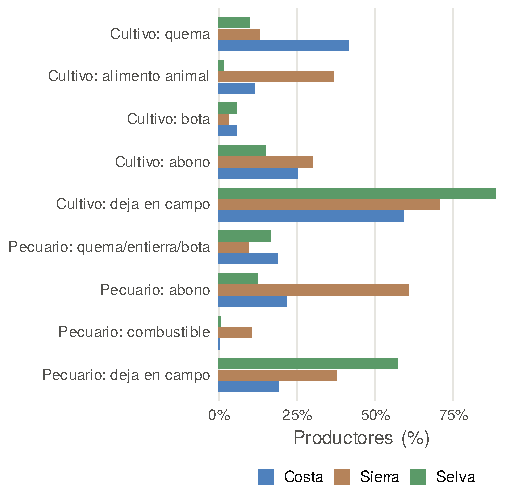
\includegraphics[width=\columnwidth]{fig02_prevalencia_region.pdf}
\caption{Prevalencia de las nueve prácticas de manejo de residuos por región natural.}
\label{fig:prev}
\end{figure}

\subsection{Número de grupos}
La Fig.~\ref{fig:k} y la Tabla~\ref{tab:seleccionk} muestran los criterios. La curva del codo desciende de forma gradual, sin un quiebre nítido, y la silueta crece con $k$, algo habitual en datos binarios de encuesta. La estabilidad, en cambio, distingue con claridad: las soluciones con $k\leq 3$ se reproducen casi idénticas entre réplicas (ARI~$=$~\ariK{} para $k=3$), mientras que con $k=4$ cae a \ariKfour. La regla de decisión seleccionó $k=\kFinal$ (Davies--Bouldin~$=$~\dbK).

\begin{figure*}[!t]
\centering
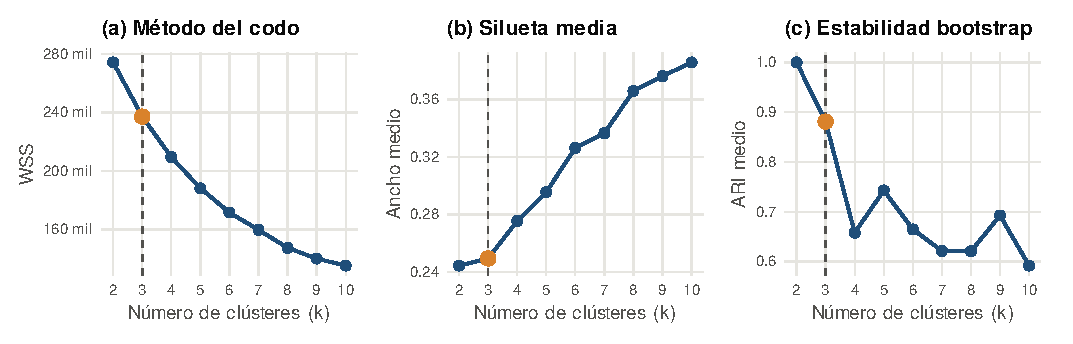
\includegraphics[width=\textwidth]{fig03_seleccion_k.pdf}
\caption{Selección del número de grupos: (a)~método del codo, (b)~silueta media y (c)~estabilidad \textit{bootstrap}. La línea discontinua marca el $k$ elegido.}
\label{fig:k}
\end{figure*}

\begin{table}[!htb]
\centering
\caption{Criterios para elegir el número de grupos}
\label{tab:seleccionk}
\footnotesize
\setlength{\tabcolsep}{3.2pt}
\begin{tabular}{@{}rrrrrrr@{}}
\toprule
$k$ & WSS & CH & DB & Silueta & ARI & Mín. (\%) \\
\midrule
2 & 274\,318 & 64\,992 & 1.865 & 0.244 & 1.000 & 42.8 \\
\rowcolor{SelRow}3 & 237\,219 & 56\,705 & 1.642 & 0.249 & 0.881 & 30.8 \\
4 & 209\,492 & 53\,598 & 1.688 & 0.275 & 0.658 & 21.3 \\
5 & 188\,154 & 51\,692 & 1.501 & 0.296 & 0.743 & 14.6 \\
6 & 171\,564 & 50\,083 & 1.399 & 0.326 & 0.665 & 10.0 \\
7 & 159\,720 & 47\,854 & 1.382 & 0.337 & 0.621 & 6.8 \\
8 & 147\,389 & 47\,372 & 1.335 & 0.366 & 0.621 & 7.3 \\
9 & 140\,023 & 45\,240 & 1.259 & 0.376 & 0.693 & 4.8 \\
10 & 135\,225 & 42\,604 & 1.275 & 0.386 & 0.592 & 4.1 \\
\bottomrule
\end{tabular}
\par\smallskip\parbox{\columnwidth}{\scriptsize WSS: suma de cuadrados intra-grupo; CH: Calinski--Harabasz ($\uparrow$); DB: Davies--Bouldin ($\downarrow$); silueta media en 10 submuestras de 8\,000 registros ($\uparrow$); ARI: estabilidad media en 20 réplicas \textit{bootstrap} ($\uparrow$); Mín.: tamaño del grupo más pequeño. Fila sombreada: $k$ elegido (ARI $\geq$ 0.80, Mín. $\geq$ 5\,\% y menor DB).}
\end{table}


\subsection{Perfiles de gestión de residuos}


La Tabla~\ref{tab:perfil} y la Fig.~\ref{fig:perfil} describen los tres grupos; la Fig.~\ref{fig:acp} los muestra en el plano de las dos primeras componentes principales.

\textit{C1 Aprovechamiento} (\pctCone\,\%). Todos sus integrantes usan el estiércol como abono (\CoRaAbono\,\%), el \CoRcAlim\,\% alimenta a sus animales con rastrojos y el \CoRcAbono\,\% los incorpora como abono; el \CoComb\,\% usa además el estiércol como combustible. Es el perfil de integración agricultura--ganadería, en el que los residuos de una actividad son insumos de la otra.

\textit{C2 Baja valorización} (\pctCtwo\,\%). Ningún integrante usa el estiércol como abono (\CtwoRaAbono\,\%) y solo el \CtwoRcAlim\,\% destina rastrojos a los animales. Concentra la quema de rastrojos (\CtwoQuema\,\%) y la eliminación inadecuada del estiércol por quema, entierro o bota (\CtwoRaInad\,\%), por lo que es el grupo con mayor riesgo ambiental y sanitario.

\textit{C3 Abandono en campo} (\pctCthree\,\%). Deja el estiércol (\CthreeRaCampo\,\%) y los rastrojos (\CthreeRcCampo\,\%) en la parcela, con poca quema (\CthreeQuema\,\%). Es un manejo pasivo: evita las emisiones de la quema, pero no aprovecha los nutrientes de forma controlada.

Las variables ilustrativas varían poco entre grupos (Tabla~\ref{tab:perfil}): el almacenamiento inadecuado de los alimentos oscila entre el \CtwoAlmInad\,\% y el \CthreeAlmInad\,\%, y la minería cercana entre el \CthreeMina\,\% y el \CoMina\,\%. La gestión de residuos y estas otras dimensiones de la inocuidad son, por tanto, relativamente independientes y requieren intervenciones propias.

\begin{figure}[!htb]
\centering
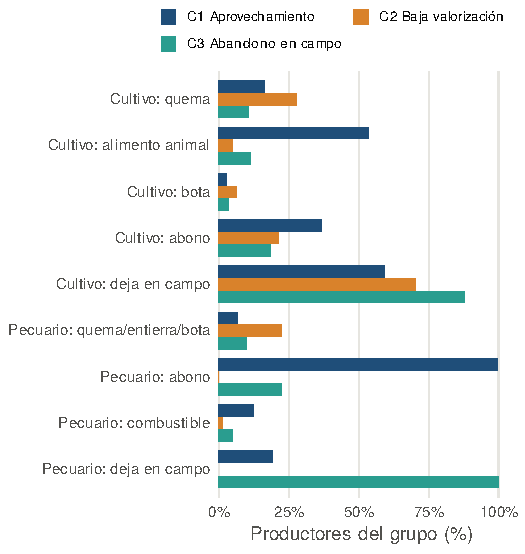
\includegraphics[width=\columnwidth]{fig07_perfil_clusters.pdf}
\caption{Perfil de los grupos: porcentaje de productores de cada grupo que realiza cada práctica.}
\label{fig:perfil}
\end{figure}

\begin{table}[!htb]
\centering
\caption{Perfil de los grupos: productores que realizan cada práctica (\%)}
\label{tab:perfil}
\footnotesize
\setlength{\tabcolsep}{3.5pt}
\begin{tabular}{@{}lrrrr@{}}
\toprule
Práctica & C1 & C2 & C3 & Total \\
$n$ & 87\,891 & 81\,408 & 75\,310 & 244\,609 \\
\midrule
\multicolumn{5}{@{}l}{\textit{Variables activas (residuos)}}\\
Cultivo: quema & 16 & 28 & 11 & 18 \\
Cultivo: alimento animal & \textbf{53} & 5 & 11 & 24 \\
Cultivo: bota & 3 & 6 & 3 & 4 \\
Cultivo: abono & 37 & 21 & 18 & 26 \\
Cultivo: deja en campo & \textbf{59} & \textbf{70} & \textbf{88} & 72 \\
Pecuario: quema/entierra/bota & 7 & 22 & 10 & 13 \\
Pecuario: abono & \textbf{100} & 0 & 22 & 43 \\
Pecuario: combustible & 12 & 1 & 5 & 6 \\
Pecuario: deja en campo & 19 & 0 & \textbf{100} & 38 \\
\midrule
\multicolumn{5}{@{}l}{\textit{Variables ilustrativas}}\\
Minería cerca del predio & 8 & 6 & 5 & 7 \\
Informado por el Estado & 7 & 7 & 6 & 7 \\
Almacén adecuado & 48 & 40 & 42 & 44 \\
Almacén inadecuado & 55 & 48 & 59 & 54 \\
Conoce identificación de alimentos & 17 & 22 & 17 & 19 \\
Certificación de calidad & 0 & 1 & 1 & 1 \\
\bottomrule
\end{tabular}
\par\smallskip\parbox{\columnwidth}{\scriptsize C1: Aprovechamiento; C2: Baja valorización; C3: Abandono en campo. En negrita, prevalencias $\geq$ 50\,\% en las variables activas.}
\end{table}


\begin{figure}[!htb]
\centering
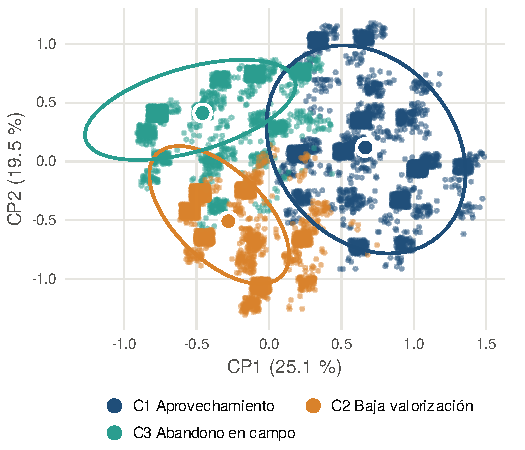
\includegraphics[width=\columnwidth]{fig06_clusters_acp.pdf}
\caption{Grupos en el plano de las dos primeras componentes principales (submuestra estratificada; los puntos se desplazan ligeramente para mostrar combinaciones repetidas). Las elipses contienen el 90\,\% de cada grupo y los círculos grandes marcan los centroides.}
\label{fig:acp}
\end{figure}

\subsection{Validación}
\begin{figure*}[!t]
\centering
\begin{minipage}[t]{0.49\textwidth}\centering
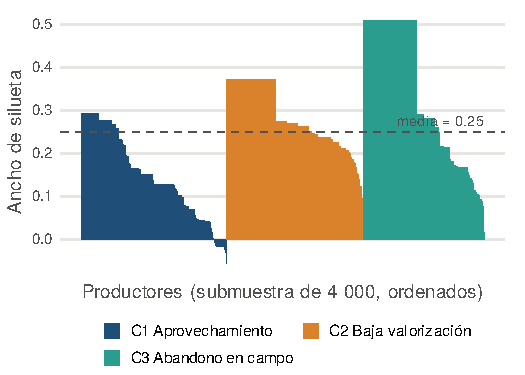
\includegraphics[width=\linewidth]{fig05_silueta.pdf}\\[-1mm]
{\footnotesize (a) Gráfico de silueta (submuestra de 4\,000 productores)}
\end{minipage}\hfill
\begin{minipage}[t]{0.49\textwidth}\centering
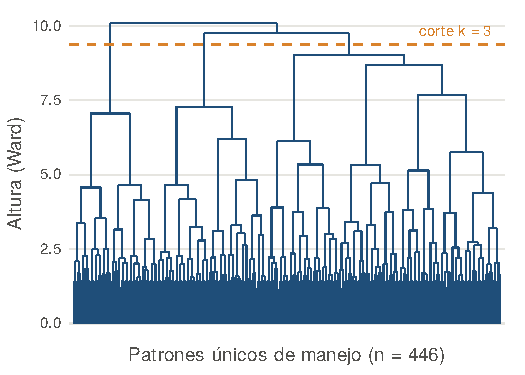
\includegraphics[width=\linewidth]{fig04_dendrograma.pdf}\\[-1mm]
{\footnotesize (b) Dendrograma de Ward (combinaciones únicas ponderadas)}
\end{minipage}
\caption{Validación de la solución con $k=3$. (a)~Ancho de silueta de cada productor, ordenado dentro de su grupo; la línea discontinua es la media. (b)~Dendrograma del método de Ward; la línea discontinua indica el corte en tres grupos.}
\label{fig:val}
\end{figure*}
La solución es estable: el ARI \textit{bootstrap} medio es \ariBoot{} (DE~\ariBootSd) y el Jaccard medio por grupo varía entre \jacMin{} y \jacMax{} (Tabla~\ref{tab:validacion}), por encima del umbral de 0.75 asociado a grupos estables~\cite{hennig2007}. La silueta media es \silK{} (Fig.~\ref{fig:val}a): C2 y C3 están bien definidos, mientras que C1 es más heterogéneo y tiene algunos productores cerca de la frontera con otros grupos. Con nueve prácticas binarias, una separación moderada es esperable; los grupos representan tendencias dominantes más que categorías aisladas.


\begin{table}[!htb]
\centering
\caption{Tamaño, cohesión y estabilidad de los grupos}
\label{tab:validacion}
\footnotesize
\setlength{\tabcolsep}{3pt}
\begin{tabular}{@{}lrrrr@{}}
\toprule
Grupo & $n$ & \% & Silueta & Jaccard \\
\midrule
C1 Aprovechamiento & 87\,891 & 35.9 & 0.147 & 0.875 \\
C2 Baja valorización & 81\,408 & 33.3 & 0.287 & 0.941 \\
C3 Abandono en campo & 75\,310 & 30.8 & 0.326 & 0.846 \\
\bottomrule
\end{tabular}
\end{table}


La concordancia entre métodos es moderada con CLARA (ARI~$=$~\ariClara) y con la tipificación $z$ (\ariZ), y casi nula con Ward (\ariWard). El dendrograma (Fig.~\ref{fig:val}b) explica esta diferencia: al cortarlo en tres grupos, Ward separa dos grupos minoritarios de combinaciones poco frecuentes y deja la mayoría de los productores en un solo grupo, en lugar de dividirla en perfiles de tamaño similar como k-means. Por su parte, la tipificación $z$ da más peso a las prácticas raras, como el uso del estiércol como combustible. Estas diferencias, consistentes con la literatura sobre tipologías agropecuarias~\cite{alvarez2018}, justifican presentar k-means como solución principal junto con sus alternativas.



\subsection{Distribución territorial y temporal}
\begin{figure*}[!t]
\centering
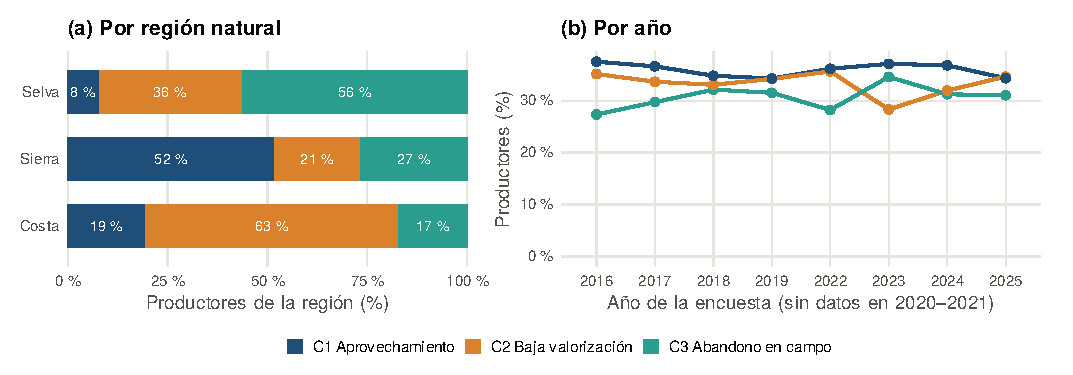
\includegraphics[width=\textwidth]{fig08_region_anio.pdf}
\caption{Distribución de los grupos (a)~por región natural y (b)~por año de la encuesta.}
\label{fig:reg}
\end{figure*}
Los grupos se asocian fuertemente con la región natural (V de Cramér~$=$~\VRegion) y con el departamento (V~$=$~\VDep), pero apenas con el año (V~$=$~\VAnio). El aprovechamiento agrupa al \SierraCone\,\% de los productores de la Sierra, coherente con la ganadería andina integrada a la agricultura; la baja valorización al \CostaCtwo\,\% de los de la Costa, donde la ganadería es menos frecuente y la quema más común; y el abandono en campo al \SelvaCthree\,\% de los de la Selva (Fig.~\ref{fig:reg}a). La composición se mantiene prácticamente estable entre 2016 y 2025 (Fig.~\ref{fig:reg}b).


\subsection{Implicaciones y limitaciones}
Los resultados sugieren políticas diferenciadas: en la Costa, reducir la quema y ofrecer alternativas de valorización de rastrojos; en la Selva, promover el compostaje o la incorporación controlada de los residuos abandonados; y en la Sierra, fortalecer las prácticas de aprovechamiento ya existentes, complementándolas con mejoras en el almacenamiento de los alimentos.

El estudio tiene limitaciones. Sin factores de expansión, los resultados no son estimaciones poblacionales. El Capítulo~600 no se aplica a los grandes productores. Las respuestas son autodeclaradas y binarias, sin información sobre volúmenes. La ENA no es un panel, por lo que no permite seguir a un mismo productor en el tiempo. Finalmente, la separación entre grupos es moderada; enfoques probabilísticos como el análisis de clases latentes podrían cuantificar la incertidumbre de la asignación individual.

\FloatBarrier
%% ==================================================================
\section{Disponibilidad de datos y código}
\noindent\textbf{Datos.} El extracto unificado del Capítulo~600 de la ENA (2014--2025; 306\,966 registros y 47 variables) y su diccionario de variables están disponibles en Zenodo bajo licencia CC~BY~4.0: \href{https://doi.org/\DOIdata}{https://doi.org/\DOIdata}~\cite{zenodo_data}. Los datos depurados, la asignación de grupo de cada registro y las tablas de resultados se regeneran a partir de ese archivo con el código descrito a continuación. Los microdatos originales son públicos en el portal del INEI~\cite{inei_ena}.

\noindent\textbf{Código.} Los scripts de R, la configuración y la fuente de este artículo están disponibles en GitHub bajo licencia MIT: \url{\GITHUB}~\cite{zenodo_code}. Siguiendo los principios FAIR~\cite{wilkinson2016,peng2011}, el análisis puede replicarse íntegramente con la semilla aleatoria indicada en el repositorio.

%% ==================================================================
\section{Conclusiones}
Los pequeños y medianos productores agropecuarios del Perú gestionan sus residuos según tres perfiles estables: \textit{aprovechamiento}, que reutiliza el estiércol y los rastrojos dentro del predio; \textit{baja valorización}, que no reutiliza el estiércol y concentra la quema y la eliminación inadecuada; y \textit{abandono en campo}, que deja ambos residuos en la parcela. Estos perfiles siguen un claro patrón territorial ---aprovechamiento en la Sierra, baja valorización en la Costa y abandono en la Selva--- y se mantuvieron estables entre 2016 y 2025.

La gestión de residuos resultó poco relacionada con otras dimensiones de la inocuidad, como el almacenamiento de los alimentos o el acceso a información estatal, cuya cobertura es baja en todos los grupos. Las políticas de manejo de residuos deberían, por ello, diferenciarse por región y por perfil de productor, y combinarse con acciones específicas de inocuidad y de información dirigidas a todos los productores.

%% ==================================================================
\section*{Declaración sobre el uso de herramientas de IA}
En la preparación del código y la redacción se utilizaron herramientas de asistencia basadas en inteligencia artificial. Los autores revisaron, ejecutaron y verificaron todo el código, los resultados y las referencias, y asumen la responsabilidad plena del contenido.

\section*{Contribución de los autores}
A.~M.~Zamora Valencia: conceptualización, análisis de datos y redacción. R.~C.~Mamani Mena, L.~E.~Cáceres Tacora y T.~K.~Butrón Maquera: revisión de la literatura, validación de resultados y revisión del manuscrito. \textit{(Ajuste estas contribuciones según el aporte real de cada autor.)}

{\footnotesize
\bibliographystyle{IEEEtran}
\bibliography{references}
}

\end{document}
